\documentclass{article}
\usepackage[utf8]{inputenc}
\usepackage{graphicx}
\usepackage{listings}

\title{CSC321 Project 2 report}
\author{g2lujinn }
\date{Due: 10pm, February 28th, 2016}

\begin{document}

\maketitle

\section*{Part 1}
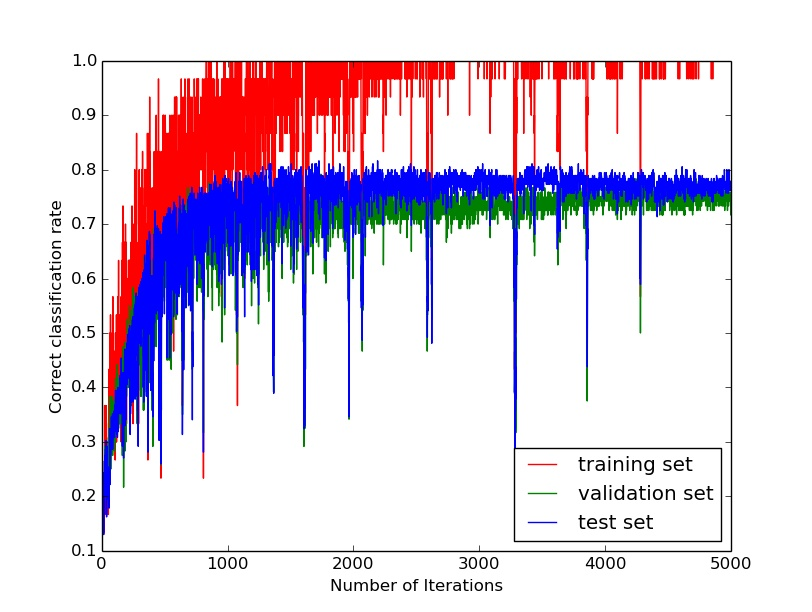
\includegraphics[scale = 0.31]{part1.png}
\indent \indent \indent This figure is generated using the code showed below:\\
\begin{lstlisting}
from pylab import *
from numpy import *
import matplotlib.pyplot as plt
import matplotlib.image as mpimg

def plot_number():
    fig = plt.figure()
    for i in range(0, 10):
        digit_name = "train" + str(i)
        for j in range(0, 10):
            plt.subplot(10,10,10*i+j+1)
            number = M[digit_name][j*10].reshape((28,28))
            imgplot = plt.imshow(number, cmap=cm.gray)
    plt.show()
plot_number()
\end{lstlisting}
\section*{Part 2}
The weights and biases are initialized as zeros since the network has no hidden layers, the code is listed below:.\\
\begin{lstlisting}
def compute_softmax(x)
	# note x is the 1x784 array from flattened 28x28 input image
  	# Initialize weights and bias, 
  	W = zeros((784, 10))
 	b = zeros((10, ))
  	# calculate outputs
 	o = dot(W.T, x)+b
  	# calculate the softmax matrix
  	return softmax(o)
\end{lstlisting}
\section*{Part 3}
The neural network used in part 3 is the same one from part 2, and below is the code used to compute the gradient of the cost function with respect to W and b.
\begin{lstlisting}
def gradient_Wb(x, W, b, y, y_):
    '''Return the gradient of the cost function with respect to W and b. Note
    that the neural network used in part 3 is the same one from part 2'''

    # gradient of cost function is p-y_, where y_ is a 10xM one-hot encoding
    # vector, and p is the softmax of y

    # Use the result of the example showed in "opt.pdf", page 7/7

    p = softmax(y)
    dCdy = p - y_

    dCdW = dot(x, dCdy.T)
    dCdb = dot(dCdy, ones((dCdy.shape[1], 1)))
    return dCdW, dCdb

\end{lstlisting}
\section*{Part 4}
Below is the source code for the finite-difference approximation function and the code for comparison:\\
\begin{lstlisting}
def finite_difference_approx(x, W, b, y_):
    '''Return the gradient w.r.t W and b using the finite difference
    approximation method'''
    # setup the differences
    h = 0.001
    dW = zeros((784, 10))
    dW[:] = h
    db = zeros((10, 1))
    db[:] = h
    
    #Estimate the derivative w.r.t W, b
    # Using the example showed in "opt.pdf", page 7/7
    dCdW = (cost(softmax(compute_y(x, W+dW, b)), y_) - \
    cost(softmax(compute_y(x, W-dW, b)), y_))/(2*dW)
    
    dCdb = (cost(softmax(compute_y(x, W, b+db)), y_) - \
    cost(softmax(compute_y(x, W, b-db)), y_))/(2*db)
    return dCdW, dCdb
    
def grad_descent(M, W, b, m, learning_rate, flag):
    '''Returns the correct gradients of W and b, it also chooses which gradient 
    method to run.
    
    Note:   this is the vectorized version of batch linear regression, 
            it takes around 1m40s to run.
    Inputs:
        M:           The MNIST dataset which contains the images to be processed.
        W:           The 784x10 weight matrix.
        b:           The 10x1 bias matrix.
        m:           The batch size.
        learning_rate:The rate initialized for computing gradients
        flag:        The variable used to indicate which gradient method to run.
    Outputs:
        W, b: The correctly computed Weight and bias matrices.
    '''
    
    W_grad = zeros((784, 10))
    b_grad = zeros((10, 1))
    # Iterate through some validation set for all the 10 digits
    for iteration in range(0, 200):
        for i in range(0, 10):
            x = vstack(M["train"+str(i)][0:m]/255.0).T # x is 784xm matrix
            y = compute_y(x, W, b) # y is now a 10xm matrix
            y_ = zeros((10, m))
            y_[i, :] = 1
            if flag == 1:
                W_temp, b_temp = gradient_Wb(x, W, b, y, y_)
            else:
                W_temp, b_temp = finite_difference_approx(x, W, b, y_)
            W_grad += W_temp
            b_grad += b_temp
            # Update the gradients at each iteration
            W -= learning_rate*(W_grad)/m
            b -= learning_rate*(b_grad)/m
    return W, b   

def compare_gradient():
    '''Print out the difference in gradient computation with function of part 3 
    and a finite difference approximation function for the same set of data'''
    # Initiate the data for comparison
    x = M["test5"][150].T/255.0
    x = x.reshape((784, 1))
    W = np.random.rand(784, 10)
    W /= W.size
    b = zeros((10, 1))
    learning_rate = 0.001


    my_dCdW, my_dCdb = grad_descent(M, W, b, 200, learning_rate, 1)
    f_dCdW, f_dCdb = grad_descent(M, W, b, 200, learning_rate, 0)
    print "The number to be predicted is: ", 5
    print "The number predicted by the normal method is:"
    print np.argmax(softmax(compute_y(x, my_dCdW, my_dCdb)))
    print "The number predicted by the finite-diff approx method is:"
    print np.argmax(softmax(compute_y(x, f_dCdW, f_dCdb)))
    print "--------------------------------------------------------------------"
    print "The precise gradient w.r.t W is:\n"
    print my_dCdW
    print "--------------------------------------------------------------------"
    print "The precise gradient w.r.t b is:\n"
    print my_dCdb
    print "--------------------------------------------------------------------"
    print "The approximate gradient w.r.t b is:\n"
    print f_dCdW
    print "--------------------------------------------------------------------"
    print "The approximate gradient w.r.t b is:\n"
    print f_dCdb
    print "--------------------------------------------------------------------"
    print "The difference of dCdW is:\n", my_dCdW-f_dCdW
    print "--------------------------------------------------------------------"
    print "The sum difference of dCdW is:\n", sum(my_dCdW-f_dCdW)
    print "--------------------------------------------------------------------"
    print "The difference of dCdb is:\n", my_dCdb-f_dCdb
compare_gradient() 

def compute_y(x, W, b):
    '''Return the output y, where y is an 10x1 matrix'''
    return dot(W.T, x)+b
\end{lstlisting}
Below is the output from both my function and a finite-difference approximation:\\
\begin{lstlisting}
In [1]: (executing lines 1 to 335 of "mnist_handout.py")
The number to be predicted is:  5
The number predicted by the normal method is:
5
The number predicted by the finite-diff approx method is:
5
--------------------------------------------------------------------
The precise gradient w.r.t W is:

[[  5.03393504e-05   4.52763533e-05   1.24392294e-04 ...,   5.91881067e-05
    1.23863127e-04   1.25511323e-04]
 [  3.52816110e-05   3.32769827e-06   6.02019109e-05 ...,   4.78036784e-05
    9.81005215e-05   5.88209944e-05]
 [  1.19926479e-04   5.12771226e-06   1.20463755e-04 ...,   1.03246147e-04
    8.29091031e-05   2.06809803e-07]
 ..., 
 [  1.09721738e-04   4.09331344e-05   1.07504584e-04 ...,   1.09017062e-04
    7.41030501e-05   9.55287592e-05]
 [  1.04654324e-04   1.24269127e-05   1.07664742e-04 ...,   6.22816815e-05
    6.61667265e-06   8.10556835e-05]
 [  1.46934351e-05   2.12913540e-05   8.99487928e-05 ...,   5.91002541e-06
    7.36297534e-05   1.21198461e-04]]
--------------------------------------------------------------------
The precise gradient w.r.t b is:

[[-3.36676189]
 [ 1.41841871]
 [ 0.36827825]
 [-2.09505652]
 [ 1.39757629]
 [ 5.10241671]
 [-0.77416412]
 [ 4.39296175]
 [-6.2888361 ]
 [-0.15483303]]
--------------------------------------------------------------------
The approximate gradient w.r.t b is:

[[  5.03393504e-05   4.52763533e-05   1.24392294e-04 ...,   5.91881067e-05
    1.23863127e-04   1.25511323e-04]
 [  3.52816110e-05   3.32769827e-06   6.02019109e-05 ...,   4.78036784e-05
    9.81005215e-05   5.88209944e-05]
 [  1.19926479e-04   5.12771226e-06   1.20463755e-04 ...,   1.03246147e-04
    8.29091031e-05   2.06809803e-07]
 ..., 
 [  1.09721738e-04   4.09331344e-05   1.07504584e-04 ...,   1.09017062e-04
    7.41030501e-05   9.55287592e-05]
 [  1.04654324e-04   1.24269127e-05   1.07664742e-04 ...,   6.22816815e-05
    6.61667265e-06   8.10556835e-05]
 [  1.46934351e-05   2.12913540e-05   8.99487928e-05 ...,   5.91002541e-06
    7.36297534e-05   1.21198461e-04]]
--------------------------------------------------------------------
The approximate gradient w.r.t b is:

[[-3.36676189]
 [ 1.41841871]
 [ 0.36827825]
 [-2.09505652]
 [ 1.39757629]
 [ 5.10241671]
 [-0.77416412]
 [ 4.39296175]
 [-6.2888361 ]
 [-0.15483303]]
--------------------------------------------------------------------
The difference of dCdW is:
[[ 0.  0.  0. ...,  0.  0.  0.]
 [ 0.  0.  0. ...,  0.  0.  0.]
 [ 0.  0.  0. ...,  0.  0.  0.]
 ..., 
 [ 0.  0.  0. ...,  0.  0.  0.]
 [ 0.  0.  0. ...,  0.  0.  0.]
 [ 0.  0.  0. ...,  0.  0.  0.]]
--------------------------------------------------------------------
The sum difference of dCdW is:
0.0
--------------------------------------------------------------------
The difference of dCdb is:
[[ 0.]
 [ 0.]
 [ 0.]
 [ 0.]
 [ 0.]
 [ 0.]
 [ 0.]
 [ 0.]
 [ 0.]
 [ 0.]]
\end{lstlisting}
\indent \indent \indent I tried several different numbers for both methods, with a training set size of 200, learning rate as 0.001, 200 iterations, and according to the output, it's obvious that there's no difference for gradient of cost function w.r.t W and b, by summing up their difference matrices I obtained zero for W matrices, so it suffices to conclude that the finite-difference approximation is correct.\\
\indent \indent \indent Note: during the computation for finite-difference approximation, I noted that learning as 0.01 produced NaN errors, so I lowered the learning rate to 0.001, and no such problem occurs anymore.
\section*{Part 5}
\indent \indent \indent Below is the learning curve for errors vs iterations.\\
\includegraphics[scale = 0.8]{errorVSiteration.png}
\clearpage
\indent \indent \indent Below is the learning curve for hitrate vs iterations, the learning rate is set to 0.01, and the highest correct classification rate achieved is about 89\%\\
\includegraphics[scale = 0.8]{hitrateVSiterationsOriginal.png}
\clearpage
\indent \indent \indent By lowering the learning rate to 0.001, the correct classification rate improved a little bit above 90\%, and below is the new learning curve for hitrate vs iterations.\\
\includegraphics[scale = 0.8]{hitrateVSiterations.png}
\clearpage
\indent Below are 20 correctly classified examples:\\
\includegraphics[scale = 0.15]{c00.png}
\includegraphics[scale = 0.15]{c01.png}
\includegraphics[scale = 0.15]{c10.png}
\includegraphics[scale = 0.15]{c11.png}
\includegraphics[scale = 0.15]{c20.png}
\includegraphics[scale = 0.15]{c21.png}
\includegraphics[scale = 0.15]{c30.png}
\includegraphics[scale = 0.15]{c31.png}
\includegraphics[scale = 0.15]{c40.png}
\includegraphics[scale = 0.15]{c41.png}
\includegraphics[scale = 0.15]{c50.png}
\includegraphics[scale = 0.15]{c51.png}
\includegraphics[scale = 0.15]{c60.png}
\includegraphics[scale = 0.15]{c61.png}
\includegraphics[scale = 0.15]{c70.png}
\includegraphics[scale = 0.15]{c71.png}
\includegraphics[scale = 0.15]{c80.png}
\includegraphics[scale = 0.15]{c81.png}
\includegraphics[scale = 0.15]{c90.png}
\includegraphics[scale = 0.15]{c91.png}
\clearpage
\indent Below are 10 incorrectly classified examples:\\
\includegraphics[scale = 0.15]{i0.png}
\indent \indent \indent This was incorrectly classified as 6\\
\includegraphics[scale = 0.15]{i1.png}
\indent \indent \indent This was incorrectly classified as 8\\
\includegraphics[scale = 0.15]{i2.png}
\indent \indent \indent This was incorrectly classified as 7\\
\includegraphics[scale = 0.15]{i3.png}
\indent \indent \indent This was incorrectly classified as 5\\
\includegraphics[scale = 0.15]{i4.png}
\indent \indent \indent This was incorrectly classified as 5\\
\includegraphics[scale = 0.15]{i5.png}
\indent \indent \indent This was incorrectly classified as 6\\
\includegraphics[scale = 0.15]{i6.png}
\indent \indent \indent This was incorrectly classified as 7\\
\includegraphics[scale = 0.15]{i7.png}
\indent \indent \indent This was incorrectly classified as 4\\
\includegraphics[scale = 0.15]{i8.png}
\indent \indent \indent This was incorrectly classified as 2\\
\includegraphics[scale = 0.15]{i9.png}
\indent \indent \indent This was incorrectly classified as 3\\
\indent Below is the code for achieving these images:
\begin{lstlisting}
def mini_batch_grad_descent(M, W, b, batch_size, learning_rate):
    '''Returns the correct gradients of W and b.
    
    Note:   this is the vectorized version of batch linear regression, 
            it takes around 1m40s to run.
    Inputs:
        M:             The MNIST dataset which contains the images to be processed.
        W:             The 784x10 weight matrix.
        b:             The 10x1 bias matrix.
        batch_size:    The mini-batch size
        learning_rate: The rate initialized for computing gradients
    Outputs:
        W, b: The correctly computed Weight and bias matrices.
        The learning curve graph for hitrate/Error vs Iterations
    '''

    W_grad = zeros((784, 10))
    b_grad = zeros((10, 1))
#     h = array([])
#     v = array([])
    # Iterate through some validation set for all the 10 digits
    for iteration in range(0, 200):
        #error = 0
        for i in range(0, 10):
            size = M["train"+str(i)].size/784
            # Use a random integer to choose where to start for mini-batch
            index = np.random.randint(0, size-batch_size)
            x = vstack(M["train"+str(i)][index:index+batch_size]/255.0).T # x is 784xm matrix
            y = compute_y(x, W, b) # y is a 10xm matrix
            y_ = zeros((10, batch_size))
            y_[i, :] = 1
            W_temp, b_temp = gradient_Wb(x, W, b, y, y_)
            W_grad += W_temp
            b_grad += b_temp
            W -= learning_rate*(W_grad)/batch_size
            b -= learning_rate*(b_grad)/batch_size
            #error += sqrt(sum((compute_softmax(x, W, b) - y_)**2))
        #Record the rate data/error data
#         rate = hitrate(W, b)
#         v = np.append(v, rate)
#         v = np.append(v, error)
#         h = np.append(h, iteration)
#         plt.plot(h, v)
    #plot the Error vs Iterations graph
#     plt.xlabel('Iterations')
#     plt.ylabel('Error')
#     plt.title('Error learning curve vs Iterations')
#     plt.show()
#     plt.xlabel('Iterations')
#     plt.ylabel('Hitrate')
#     plt.title('Hitrate learning curve vs Iterations')
#     plt.show()
    return W, b

def plot_rateVSiteration():
    '''This function plots the hitrate vs iteration learning curve, it can 
    also be modified to produce the images for part 5'''
    # Initiate the data for comparison
    W = np.random.rand(784, 10)
    W /= W.size
    b = zeros((10, 1))
    learning_rate = 0.001
    m = 50
    dCdW, dCdb = mini_batch_grad_descent(M, W, b, m, learning_rate)
    # use two lists to grab 20 correctly classified and 10 incorrectly classifed
    # digits
    max_count_correct = []
    # max_count_incorrect = []
    # incorrect_digits = []
    # Iterate through some test set for all the 10 digits
    # The loop is needed to gather individual information for digits
    for i in range(0, 10):
        counter = 0
        size = M["test"+str(i)].size/784
        for j in range(0, size):
            x = (M["test"+str(i)][j]/255.0).T
            x = x.reshape((784, 1))
            digit = argmax(compute_softmax(x, dCdW, dCdb))
            # Grab the disired images
            if digit - i == 0 and len(max_count_correct) < 20 and counter < 2:
                max_count_correct.append((i, j))
                counter += 1
            # if digit - i != 0 and len(max_count_incorrect) < 10:
            #     max_count_incorrect.append((i, j))
            #     incorrect_digits.append(digit)

    for item in max_count_correct:
    # for item in max_count_incorrect:
        imshow(M["train"+str(item[0])][item[1]].reshape((28,28)), cmap=cm.gray)
        # print "The incorrectly predicted digit is: ", incorrect_digits[0]
        show()
plot_rateVSiteration()
\end{lstlisting}
\section*{Part 6}
\includegraphics[scale = 0.3]{heat0.png}
\includegraphics[scale = 0.3]{heat1.png}
\includegraphics[scale = 0.3]{heat2.png}
\includegraphics[scale = 0.3]{heat3.png}
\includegraphics[scale = 0.3]{heat4.png}
\includegraphics[scale = 0.3]{heat5.png}
\includegraphics[scale = 0.3]{heat6.png}
\includegraphics[scale = 0.3]{heat7.png}
\includegraphics[scale = 0.3]{heat8.png}
\includegraphics[scale = 0.3]{heat9.png}
\indent Above are heatmaps for all ten digits, apparently, the red part (with higher values) represents the features for each digit.\\
\section*{Part 7}
Below is the source code implemented for computing the gradients in both ways:\\
\begin{lstlisting}
def compute_p_hidden(x, W0, b0, W1, b1):
    '''Return only the final output of the network'''
    L0 = tanh_layer(x, W0, b0)
    L1 = tanh_layer(L0, W1, b1)
    output = softmax(L1)
    return output

def gradient_Hidden(x, W0, b0, W1, b1, L0, y, p, y_):
    '''Return the gradient of the cost function with respect to W and b. Note
    that the neural network used in part 3 is the same one from part 2'''

    # gradient of cost function is p-y_, where y_ is a 10xM one-hot encoding
    # vector, and p is the softmax of y

    # Use the result of the example showed in "opt.pdf", page 7/7
    dCdy = p - y_
    dCdL0 = dot(W1, (1 - y**2)*dCdy)
    dCdW1 = dot(L0, ((1 - y**2)*dCdy).T) # compute gradient w.r.t hidden layer 1
    dCdW0 = dot(x, ((1-L0**2)*dCdL0).T) # compute gradient w.r.t hidden layer 0
    
    dCdb0 = dot(dCdL0, ones((dCdL0.shape[0], 1)))
    dCdb1 = dot(dCdy, ones((dCdy.shape[1], 1)))
    return dCdW0, dCdW1, dCdb0, dCdb1

def finite_difference_approx_hidden(x, W0, b0, W1, b1, L0, y, y_):
    '''Return the gradient w.r.t W and b using the finite difference
    approximation method'''
    # setup the differences
    h = 0.001
    dy = zeros((10, 300))
    dy[:] = h
    dL0 = zeros((300, 300))
    dL0[:] = h
    dW0 = zeros((784, 300))
    dW0[:] = h
    dW1 = zeros((300, 10))
    dW1[:] = h
    db0 = zeros((300, 1))
    db0[:] = h
    db1 = zeros((10, 1))
    db1[:] = h

    #Estimate the derivative w.r.t W, b
    # Using the example showed in "opt.pdf", page 7/7
    dCdW0 = (cost(softmax(tanh_layer(tanh_layer(x, W0+dW0, b0), W1, b1)), y_) - \
            cost(softmax(tanh_layer(tanh_layer(x, W0-dW0, b0), W1, b1)), y_) )/(2*h)

    dCdW1 = (cost(softmax(tanh_layer(L0, W1+dW1, b1)), y_) - \
            cost(softmax(tanh_layer(L0, W1-dW1, b1)), y_) )/(2*h) 
    
    dCdb0 = (cost(softmax(tanh_layer(tanh_layer(x, W0, b0+db0), W1, b1)), y_) - \
            cost(softmax(tanh_layer(tanh_layer(x, W0, b0-db0), W1, b1)), y_) )/(2*h)
    dCdb1 = (cost(softmax(tanh_layer(L0, W1, b1+db1)), y_) - \
            cost(softmax(tanh_layer(L0, W1, b1-db1)), y_) )/(2*h)

    return dCdW0, dCdW1, dCdb0, dCdb1

def grad_descent_hidden(M, m, learning_rate, flag):
    '''Returns the correct gradients of W0, W1 and b0, b1, it also chooses which gradient 
    method to run, this function uses a neural network with a hidden layer.
    
    Note:   this is the vectorized version of batch linear regression, 
            it takes around 1m40s to run.
    Inputs:
        M:           The MNIST dataset which contains the images to be processed.
        m:           The batch size. Now it's initialized as 300
        learning_rate:The rate initialized for computing gradients
        flag:        The variable used to indicate which gradient method to run.
    Outputs:
        W, b: The correctly computed Weight and bias matrices.
    '''
    W0 = init_W0
    W1 = init_W1
    b0 = init_b0
    b1 = init_b1
    W0_grad = zeros((784, W0.shape[1]))
    b0_grad = zeros((b0.shape[0], 1))    
    W1_grad = zeros((W1.shape[0], W1.shape[1]))
    b1_grad = zeros((b1.shape[0], 1))
    # Iterate through some validation set for all the 10 digits
    for iteration in range(0, 200):
        for i in range(0, 10):
            x = vstack(M["train"+str(i)][0:m]/255.).T # x is 784xm matrix
            y_ = zeros((10, m))
            y_[i, :] = 1
            if flag == 1: # Choose which method to run
                L0, y, p = forward(x, W0, b0, W1, b1) # compute the hidden layer and softmax p
                W0_temp, W1_temp, b0_temp, b1_temp = \
                gradient_Hidden(x, W0, b0, W1, b1, L0, y, p, y_)
            else:
                W0_temp, W1_temp, b0_temp, b1_temp = \
                finite_difference_approx_hidden(x, W0, b0, W1, b1, y_)
            W0_grad += W0_temp
            b0_grad += b0_temp
            W1_grad += W1_temp
            b1_grad += b1_temp
            # Update the gradients at each iteration
            W0 -= learning_rate*(W0_grad)/m
            b0 -= learning_rate*(b0_grad)/m
            W1 -= learning_rate*(W1_grad)/m
            b1 -= learning_rate*(b1_grad)/m
    return W0, b0, W1, b1
\end{lstlisting}
\indent The new neural network is computed in following steps:\\
\indent \indent \indent $y_i = 1, y_j = 0$ \textit{for} $i\neq j$\\
\indent \indent \indent $L0_j = tanh(W0_j^T\cdot x_j+b0_j)$\\
\indent \indent \indent $L1_j = tanh(W1_j^T\cdot L0_j+b1_j)$\\
\indent \indent \indent $p_i = \frac{e^{L1_i}}{\Sigma_{j}e^{L1_j}}$\\
\indent \indent \indent $C = -\Sigma_{j}y_jlog L1_j$
\section*{Part 8}
Below is the source code used to output the W0, b0, W1, b1:\\
\begin{lstlisting}
# Initialize data
snapshot = cPickle.load(open("/h/u16/g2/00/g2lujinn/Downloads/CSC321/Assignment 2/snapshot50.pkl"))
init_W0 = snapshot["W0"]
init_b0 = snapshot["b0"].reshape((300,1))
init_W1 = snapshot["W1"]
init_b1 = snapshot["b1"].reshape((10,1))

def compare_gradient_hidden():
    '''Print out the difference in gradient computation with function of part 3 
    and a finite difference approximation function for the same set of data'''
    # Initiate the data for comparison
    learning_rate = 0.01

    my_dCdW0, my_dCdb0, my_dCdW1, my_dCdb1 = grad_descent_hidden(M, 300, learning_rate, 1)
    f_dCdW0, f_dCdb0, f_dCdW1, f_dCdb1 = grad_descent_hidden(M, 300, learning_rate, 0)
    print "--------------------------------------------------------------------"
    print "The precise gradient w.r.t W is:\n"
    print my_dCdW0, my_dCdW1
    print "--------------------------------------------------------------------"
    print "The precise gradient w.r.t b is:\n"
    print my_dCdb0, my_dCdb1
    print "--------------------------------------------------------------------"
    print "The approximate gradient w.r.t b is:\n"
    print f_dCdW0, f_dCdW1
    print "--------------------------------------------------------------------"
    print "The approximate gradient w.r.t b is:\n"
    print f_dCdb0, f_dCdb1
    print "--------------------------------------------------------------------"
    print "The difference of dCdW0 is:\n", my_dCdW0-f_dCdW0
    print "--------------------------------------------------------------------"
    print "The difference of dCdW1 is:\n", my_dCdW1-f_dCdW1
    print "--------------------------------------------------------------------"
    print "The sum difference of dCdb0 is:\n", sum(my_dCdb0-f_dCdb0)
    print "--------------------------------------------------------------------"
    print "The sum difference of dCdb1 is:\n", sum(my_dCdb1-f_dCdb1)
compare_gradient_hidden() 
\end{lstlisting}
And below is the output, note that I used learning rate of 0.01:
\begin{lstlisting}
--------------------------------------------------------------------
The precise gradient w.r.t W is:

[[ 217.5975647   217.60012817  217.60003662 ...,  217.6089325   217.59420776
   217.58575439]
 [ 217.59173584  217.60006714  217.60437012 ...,  217.61000061
   217.59158325  217.58280945]
 [ 217.60205078  217.59140015  217.60717773 ...,  217.60295105
   217.58905029  217.59713745]
 ..., 
 [ 217.5846405   217.60539246  217.59477234 ...,  217.58512878
   217.57995605  217.58787537]
 [ 217.59368896  217.59579468  217.59373474 ...,  217.59700012
   217.58081055  217.60188293]
 [ 217.60121155  217.58311462  217.59959412 ...,  217.59796143
   217.59432983  217.60105896]] [[-55.71722031 -48.79885864 -49.02945709 ..., -50.3337822  -51.50911713
  -55.62484741]
 [-52.99531937 -50.72525024 -49.93320465 ..., -49.73569489 -52.87190628
  -46.94050598]
 [-50.5851593  -50.35341644 -50.32669449 ..., -49.81040192 -52.5493927
  -48.11484909]
 ..., 
 [-54.25477219 -51.19381714 -48.95261383 ..., -50.9563942  -51.64023209
  -53.49124146]
 [-55.91595459 -50.09132004 -50.48883438 ..., -50.95417023 -52.13952255
  -52.89031601]
 [-51.39916229 -49.30364609 -49.91474152 ..., -45.62763596 -50.42440796
  -45.47509766]]
--------------------------------------------------------------------
The precise gradient w.r.t b is:

[[ 3.53321838]
 [ 3.03172994]
 [ 3.3192153 ]
 [ 3.29898882]
 [ 3.59854507]
 [ 3.54130769]
 [ 3.08872247]
 [ 3.19871402]
 [ 3.07319522]
 [ 3.28504658]
 [ 4.23672724]
 [ 3.29277062]
 [ 3.27823758]
 [ 3.30368304]
 [ 3.24941826]
 [ 3.10384798]
 [ 2.4323101 ]
 [ 3.34753609]
 [ 3.24983597]
 [ 3.83824301]
 [ 3.18578219]
 [ 4.33447552]
 [ 2.68902874]
 [ 3.32252049]
 [ 3.10632443]
 [ 4.04379988]
 [ 3.31628919]
 [ 3.07665348]
 [ 3.06976652]
 [ 3.20018435]
 [ 3.25705218]
 [ 3.26560187]
 [ 3.11947703]
 [ 3.24204373]
 [ 4.04339981]
 [ 2.77846217]
 [ 4.11631823]
 [ 3.07881069]
 [ 2.86438799]
 [ 3.25692439]
 [ 2.92789507]
 [ 4.81010437]
 [ 4.14207029]
 [ 3.06172848]
 [ 3.11475539]
 [ 4.71038151]
 [ 2.87999129]
 [ 3.48837161]
 [ 2.99249816]
 [ 3.25165439]
 [ 3.51587462]
 [ 4.31166506]
 [ 3.35798144]
 [ 3.16712952]
 [ 2.99602151]
 [ 3.64567614]
 [ 3.63842869]
 [ 3.25308084]
 [ 3.40219021]
 [ 3.354182  ]
 [ 3.39602399]
 [ 3.31995821]
 [ 3.1561408 ]
 [ 3.17244196]
 [ 3.56582808]
 [ 5.76788807]
 [ 3.31645036]
 [ 3.23406553]
 [ 3.19377804]
 [ 3.23557258]
 [ 3.41482639]
 [ 3.17449427]
 [ 3.68943071]
 [ 2.96213174]
 [ 3.05650449]
 [ 3.34691548]
 [ 3.213624  ]
 [ 4.02779436]
 [ 4.02403259]
 [ 3.06070161]
 [ 3.04435539]
 [ 3.55455899]
 [ 3.34896302]
 [ 4.14555502]
 [ 2.92227173]
 [ 3.49389482]
 [ 2.90588498]
 [ 3.36108398]
 [ 3.16160583]
 [ 2.96564555]
 [ 4.25850248]
 [ 3.04074979]
 [ 3.44229698]
 [ 3.17479849]
 [ 3.12798882]
 [ 1.85058045]
 [ 3.54006124]
 [ 3.2393074 ]
 [ 3.24614882]
 [ 3.09712863]
 [ 4.37106657]
 [ 3.02471375]
 [ 3.21660233]
 [ 3.289078  ]
 [ 2.99000764]
 [ 3.01861596]
 [ 3.21905422]
 [ 4.27250099]
 [ 3.82713556]
 [ 3.66305685]
 [ 3.94152665]
 [ 2.33584785]
 [ 3.07685328]
 [ 2.98463655]
 [ 4.191998  ]
 [ 3.19656014]
 [ 3.41449142]
 [ 3.26841259]
 [ 2.94522452]
 [ 3.32796025]
 [ 4.03969669]
 [ 3.37651777]
 [ 3.47141981]
 [ 3.66627049]
 [ 3.98846173]
 [ 3.17936945]
 [ 2.85794187]
 [ 3.13974118]
 [ 3.33521986]
 [ 3.03547931]
 [ 3.11235976]
 [ 3.41464496]
 [ 3.34423614]
 [ 3.09847403]
 [ 2.93942928]
 [ 3.06943607]
 [ 2.93524551]
 [ 2.99811029]
 [ 3.15614057]
 [ 3.31783891]
 [ 3.09770083]
 [ 2.92441297]
 [ 3.20882583]
 [ 3.32761884]
 [ 2.89240408]
 [ 3.79797029]
 [ 3.68484545]
 [ 4.83170366]
 [ 3.96034789]
 [ 3.27822495]
 [ 2.36389279]
 [ 2.58781457]
 [ 3.11464   ]
 [ 3.15782523]
 [ 3.55991411]
 [ 3.41482544]
 [ 3.83804917]
 [ 3.99363947]
 [ 2.66103196]
 [ 3.58155966]
 [ 3.43489313]
 [ 4.29465103]
 [ 3.7193377 ]
 [ 3.235636  ]
 [ 3.40579009]
 [ 3.20193362]
 [ 3.19149995]
 [ 3.20959854]
 [ 3.30155468]
 [ 4.19891405]
 [ 3.29390359]
 [ 3.6690011 ]
 [ 3.1868    ]
 [ 3.1114974 ]
 [ 3.36833143]
 [ 3.68398046]
 [ 2.99856496]
 [ 3.1204443 ]
 [ 3.67180133]
 [ 3.04633737]
 [ 3.53254557]
 [ 3.92833567]
 [ 3.30068588]
 [ 4.4813838 ]
 [ 3.6231792 ]
 [ 2.88490629]
 [ 4.1390295 ]
 [ 3.26672006]
 [ 3.96912313]
 [ 2.97364116]
 [ 4.47831154]
 [ 3.18906116]
 [ 4.14361   ]
 [ 3.22509551]
 [ 3.81834292]
 [ 2.12239623]
 [ 3.14739323]
 [ 2.9854784 ]
 [ 3.38031197]
 [ 3.48407793]
 [ 3.75833344]
 [ 3.06017923]
 [ 3.09862137]
 [ 3.05307126]
 [ 3.38844323]
 [ 3.2954495 ]
 [ 3.1857996 ]
 [ 3.18085766]
 [ 3.09351826]
 [ 3.2845552 ]
 [ 3.10071826]
 [ 2.68770957]
 [ 2.85670543]
 [ 2.98102498]
 [ 3.22220159]
 [ 3.40658236]
 [ 2.70667148]
 [ 3.31894803]
 [ 3.11802983]
 [ 5.00901127]
 [ 3.30347395]
 [ 3.3453424 ]
 [ 3.07935333]
 [ 3.4291091 ]
 [ 2.97909832]
 [ 3.35349965]
 [ 4.91949749]
 [ 3.99045515]
 [ 3.86424899]
 [ 3.44831634]
 [ 2.978158  ]
 [ 3.67574906]
 [ 3.21103573]
 [ 3.11729813]
 [ 3.24606991]
 [ 3.22929811]
 [ 2.95029116]
 [ 3.76254487]
 [ 2.50679374]
 [ 3.92135072]
 [ 3.85040736]
 [ 3.162534  ]
 [ 3.72688866]
 [ 3.23251677]
 [ 3.43958712]
 [ 3.519804  ]
 [ 2.93117142]
 [ 2.79480982]
 [ 3.5801785 ]
 [ 3.61740971]
 [ 3.38150573]
 [ 3.42600155]
 [ 3.23715878]
 [ 3.78435826]
 [ 3.4878583 ]
 [ 2.99853516]
 [ 3.24493313]
 [ 3.47289228]
 [ 3.14963961]
 [ 2.93928909]
 [ 3.07610297]
 [ 3.78207898]
 [ 3.12091422]
 [ 3.65415835]
 [ 3.56660795]
 [ 3.04681468]
 [ 3.50793886]
 [ 2.95777202]
 [ 4.52738857]
 [ 3.29555774]
 [ 2.63968086]
 [ 3.27058506]
 [ 3.80318117]
 [ 3.25243378]
 [ 2.96383619]
 [ 3.21760845]
 [ 3.21644211]
 [ 3.06313396]
 [ 3.26918173]
 [ 3.29005814]
 [ 3.56245542]
 [ 3.1124413 ]
 [ 3.03518319]
 [ 3.75687432]
 [ 3.13432479]
 [ 3.93580961]
 [ 3.30129004]
 [ 3.18585849]
 [ 3.08653617]
 [ 3.07878351]
 [ 4.50219154]
 [ 3.59855819]
 [ 3.36740708]
 [ 3.23916221]
 [ 2.86245847]
 [ 3.21614552]
 [ 4.89559317]
 [ 3.26885796]
 [ 3.49913239]
 [ 2.42297888]] [[ -56.64134979]
 [   2.59951496]
 [  -3.50100923]
 [  -2.37593675]
 [   3.41278458]
 [ -20.36026382]
 [   3.00623894]
 [  25.93379784]
 [ 164.50015259]
 [-112.88748169]]
--------------------------------------------------------------------
The approximate gradient w.r.t b is:

[[ 217.5975647   217.60012817  217.60003662 ...,  217.6089325   217.59420776
   217.58575439]
 [ 217.59173584  217.60006714  217.60437012 ...,  217.61000061
   217.59158325  217.58280945]
 [ 217.60205078  217.59140015  217.60717773 ...,  217.60295105
   217.58905029  217.59713745]
 ..., 
 [ 217.5846405   217.60539246  217.59477234 ...,  217.58512878
   217.57995605  217.58787537]
 [ 217.59368896  217.59579468  217.59373474 ...,  217.59700012
   217.58081055  217.60188293]
 [ 217.60121155  217.58311462  217.59959412 ...,  217.59796143
   217.59432983  217.60105896]] [[-55.71722031 -48.79885864 -49.02945709 ..., -50.3337822  -51.50911713
  -55.62484741]
 [-52.99531937 -50.72525024 -49.93320465 ..., -49.73569489 -52.87190628
  -46.94050598]
 [-50.5851593  -50.35341644 -50.32669449 ..., -49.81040192 -52.5493927
  -48.11484909]
 ..., 
 [-54.25477219 -51.19381714 -48.95261383 ..., -50.9563942  -51.64023209
  -53.49124146]
 [-55.91595459 -50.09132004 -50.48883438 ..., -50.95417023 -52.13952255
  -52.89031601]
 [-51.39916229 -49.30364609 -49.91474152 ..., -45.62763596 -50.42440796
  -45.47509766]]
--------------------------------------------------------------------
The approximate gradient w.r.t b is:

[[ 3.53321838]
 [ 3.03172994]
 [ 3.3192153 ]
 [ 3.29898882]
 [ 3.59854507]
 [ 3.54130769]
 [ 3.08872247]
 [ 3.19871402]
 [ 3.07319522]
 [ 3.28504658]
 [ 4.23672724]
 [ 3.29277062]
 [ 3.27823758]
 [ 3.30368304]
 [ 3.24941826]
 [ 3.10384798]
 [ 2.4323101 ]
 [ 3.34753609]
 [ 3.24983597]
 [ 3.83824301]
 [ 3.18578219]
 [ 4.33447552]
 [ 2.68902874]
 [ 3.32252049]
 [ 3.10632443]
 [ 4.04379988]
 [ 3.31628919]
 [ 3.07665348]
 [ 3.06976652]
 [ 3.20018435]
 [ 3.25705218]
 [ 3.26560187]
 [ 3.11947703]
 [ 3.24204373]
 [ 4.04339981]
 [ 2.77846217]
 [ 4.11631823]
 [ 3.07881069]
 [ 2.86438799]
 [ 3.25692439]
 [ 2.92789507]
 [ 4.81010437]
 [ 4.14207029]
 [ 3.06172848]
 [ 3.11475539]
 [ 4.71038151]
 [ 2.87999129]
 [ 3.48837161]
 [ 2.99249816]
 [ 3.25165439]
 [ 3.51587462]
 [ 4.31166506]
 [ 3.35798144]
 [ 3.16712952]
 [ 2.99602151]
 [ 3.64567614]
 [ 3.63842869]
 [ 3.25308084]
 [ 3.40219021]
 [ 3.354182  ]
 [ 3.39602399]
 [ 3.31995821]
 [ 3.1561408 ]
 [ 3.17244196]
 [ 3.56582808]
 [ 5.76788807]
 [ 3.31645036]
 [ 3.23406553]
 [ 3.19377804]
 [ 3.23557258]
 [ 3.41482639]
 [ 3.17449427]
 [ 3.68943071]
 [ 2.96213174]
 [ 3.05650449]
 [ 3.34691548]
 [ 3.213624  ]
 [ 4.02779436]
 [ 4.02403259]
 [ 3.06070161]
 [ 3.04435539]
 [ 3.55455899]
 [ 3.34896302]
 [ 4.14555502]
 [ 2.92227173]
 [ 3.49389482]
 [ 2.90588498]
 [ 3.36108398]
 [ 3.16160583]
 [ 2.96564555]
 [ 4.25850248]
 [ 3.04074979]
 [ 3.44229698]
 [ 3.17479849]
 [ 3.12798882]
 [ 1.85058045]
 [ 3.54006124]
 [ 3.2393074 ]
 [ 3.24614882]
 [ 3.09712863]
 [ 4.37106657]
 [ 3.02471375]
 [ 3.21660233]
 [ 3.289078  ]
 [ 2.99000764]
 [ 3.01861596]
 [ 3.21905422]
 [ 4.27250099]
 [ 3.82713556]
 [ 3.66305685]
 [ 3.94152665]
 [ 2.33584785]
 [ 3.07685328]
 [ 2.98463655]
 [ 4.191998  ]
 [ 3.19656014]
 [ 3.41449142]
 [ 3.26841259]
 [ 2.94522452]
 [ 3.32796025]
 [ 4.03969669]
 [ 3.37651777]
 [ 3.47141981]
 [ 3.66627049]
 [ 3.98846173]
 [ 3.17936945]
 [ 2.85794187]
 [ 3.13974118]
 [ 3.33521986]
 [ 3.03547931]
 [ 3.11235976]
 [ 3.41464496]
 [ 3.34423614]
 [ 3.09847403]
 [ 2.93942928]
 [ 3.06943607]
 [ 2.93524551]
 [ 2.99811029]
 [ 3.15614057]
 [ 3.31783891]
 [ 3.09770083]
 [ 2.92441297]
 [ 3.20882583]
 [ 3.32761884]
 [ 2.89240408]
 [ 3.79797029]
 [ 3.68484545]
 [ 4.83170366]
 [ 3.96034789]
 [ 3.27822495]
 [ 2.36389279]
 [ 2.58781457]
 [ 3.11464   ]
 [ 3.15782523]
 [ 3.55991411]
 [ 3.41482544]
 [ 3.83804917]
 [ 3.99363947]
 [ 2.66103196]
 [ 3.58155966]
 [ 3.43489313]
 [ 4.29465103]
 [ 3.7193377 ]
 [ 3.235636  ]
 [ 3.40579009]
 [ 3.20193362]
 [ 3.19149995]
 [ 3.20959854]
 [ 3.30155468]
 [ 4.19891405]
 [ 3.29390359]
 [ 3.6690011 ]
 [ 3.1868    ]
 [ 3.1114974 ]
 [ 3.36833143]
 [ 3.68398046]
 [ 2.99856496]
 [ 3.1204443 ]
 [ 3.67180133]
 [ 3.04633737]
 [ 3.53254557]
 [ 3.92833567]
 [ 3.30068588]
 [ 4.4813838 ]
 [ 3.6231792 ]
 [ 2.88490629]
 [ 4.1390295 ]
 [ 3.26672006]
 [ 3.96912313]
 [ 2.97364116]
 [ 4.47831154]
 [ 3.18906116]
 [ 4.14361   ]
 [ 3.22509551]
 [ 3.81834292]
 [ 2.12239623]
 [ 3.14739323]
 [ 2.9854784 ]
 [ 3.38031197]
 [ 3.48407793]
 [ 3.75833344]
 [ 3.06017923]
 [ 3.09862137]
 [ 3.05307126]
 [ 3.38844323]
 [ 3.2954495 ]
 [ 3.1857996 ]
 [ 3.18085766]
 [ 3.09351826]
 [ 3.2845552 ]
 [ 3.10071826]
 [ 2.68770957]
 [ 2.85670543]
 [ 2.98102498]
 [ 3.22220159]
 [ 3.40658236]
 [ 2.70667148]
 [ 3.31894803]
 [ 3.11802983]
 [ 5.00901127]
 [ 3.30347395]
 [ 3.3453424 ]
 [ 3.07935333]
 [ 3.4291091 ]
 [ 2.97909832]
 [ 3.35349965]
 [ 4.91949749]
 [ 3.99045515]
 [ 3.86424899]
 [ 3.44831634]
 [ 2.978158  ]
 [ 3.67574906]
 [ 3.21103573]
 [ 3.11729813]
 [ 3.24606991]
 [ 3.22929811]
 [ 2.95029116]
 [ 3.76254487]
 [ 2.50679374]
 [ 3.92135072]
 [ 3.85040736]
 [ 3.162534  ]
 [ 3.72688866]
 [ 3.23251677]
 [ 3.43958712]
 [ 3.519804  ]
 [ 2.93117142]
 [ 2.79480982]
 [ 3.5801785 ]
 [ 3.61740971]
 [ 3.38150573]
 [ 3.42600155]
 [ 3.23715878]
 [ 3.78435826]
 [ 3.4878583 ]
 [ 2.99853516]
 [ 3.24493313]
 [ 3.47289228]
 [ 3.14963961]
 [ 2.93928909]
 [ 3.07610297]
 [ 3.78207898]
 [ 3.12091422]
 [ 3.65415835]
 [ 3.56660795]
 [ 3.04681468]
 [ 3.50793886]
 [ 2.95777202]
 [ 4.52738857]
 [ 3.29555774]
 [ 2.63968086]
 [ 3.27058506]
 [ 3.80318117]
 [ 3.25243378]
 [ 2.96383619]
 [ 3.21760845]
 [ 3.21644211]
 [ 3.06313396]
 [ 3.26918173]
 [ 3.29005814]
 [ 3.56245542]
 [ 3.1124413 ]
 [ 3.03518319]
 [ 3.75687432]
 [ 3.13432479]
 [ 3.93580961]
 [ 3.30129004]
 [ 3.18585849]
 [ 3.08653617]
 [ 3.07878351]
 [ 4.50219154]
 [ 3.59855819]
 [ 3.36740708]
 [ 3.23916221]
 [ 2.86245847]
 [ 3.21614552]
 [ 4.89559317]
 [ 3.26885796]
 [ 3.49913239]
 [ 2.42297888]] [[ -56.64134979]
 [   2.59951496]
 [  -3.50100923]
 [  -2.37593675]
 [   3.41278458]
 [ -20.36026382]
 [   3.00623894]
 [  25.93379784]
 [ 164.50015259]
 [-112.88748169]]
--------------------------------------------------------------------
The difference of dCdW0 is:
[[ 0.  0.  0. ...,  0.  0.  0.]
 [ 0.  0.  0. ...,  0.  0.  0.]
 [ 0.  0.  0. ...,  0.  0.  0.]
 ..., 
 [ 0.  0.  0. ...,  0.  0.  0.]
 [ 0.  0.  0. ...,  0.  0.  0.]
 [ 0.  0.  0. ...,  0.  0.  0.]]
--------------------------------------------------------------------
The difference of dCdW1 is:
[[ 0.  0.  0. ...,  0.  0.  0.]
 [ 0.  0.  0. ...,  0.  0.  0.]
 [ 0.  0.  0. ...,  0.  0.  0.]
 ..., 
 [ 0.  0.  0. ...,  0.  0.  0.]
 [ 0.  0.  0. ...,  0.  0.  0.]
 [ 0.  0.  0. ...,  0.  0.  0.]]
--------------------------------------------------------------------
The sum difference of dCdb0 is:
0.0
--------------------------------------------------------------------
The sum difference of dCdb1 is:
0.0
\end{lstlisting}
\section*{Part 9}
\indent \indent Below is the code for part 9:
\begin{lstlisting}
def hitrate_hidden(dCdW0, dCdb0, dCdW1, dCdb1):
    '''Return the classification rate for any given W, b gradient
    This function calculates the hitrate by using all available test cases.'''

    hit = 0.0
    total = 0.0

    # Iterate through some test set for all the 10 digits
    for i in range(0, 10):
        size = M["test"+str(i)].size/784
        x = (M["test"+str(i)][0:size]/255.0).T
        # Vectorize the hitrate computation
        digit_matrix = argmax(compute_p_hidden(x, dCdW0, dCdb0, dCdW1, dCdb1), axis = 0)
        digit_matrix = digit_matrix.reshape((1, size))
        
        targets = zeros((digit_matrix.shape[0], digit_matrix.shape[1]))
        targets[:] = i
        
        result = digit_matrix - targets
        hit += result.shape[1] - np.count_nonzero(result)
        total += digit_matrix.shape[1]
    return hit/total

def mini_batch_grad_descent_hidden(M, W0, b0, W1, b1, batch_size, learning_rate):
    '''Returns the correct gradients of W and b.
    
    Note:   this is the vectorized version of batch linear regression, 
            it takes around 1m40s to run.
    Inputs:
        M:             The MNIST dataset which contains the images to be processed.
        batch_size:    The mini-batch size
        learning_rate: The rate initialized for computing gradients
    Outputs:
        W, b: The correctly computed Weight and bias matrices.
    '''

    W0_grad = zeros((784, W0.shape[1]))
    b0_grad = zeros((b0.shape[0], 1))    
    W1_grad = zeros((W1.shape[0], W1.shape[1]))
    b1_grad = zeros((b1.shape[0], 1))
    h = array([])
    v = array([])
    # Iterate through some validation set for all the 10 digits
    for iteration in range(0, 20000): # Iterations of 20000 achieves 95% hitrate
        error = 0
        for i in range(0, 10):
            size = M["train"+str(i)].size/784
            # Use a random integer to choose where to start for mini-batch
            index = np.random.randint(0, size-batch_size)
            x = vstack(M["train"+str(i)][index:index+batch_size]/255.).T # x is 784xm matrix
            y_ = zeros((10, batch_size))
            y_[i, :] = 1
            L0, y, p = forward(x, W0, b0, W1, b1) # compute the hidden layer and softmax p
            W0_temp, W1_temp, b0_temp, b1_temp = \
                gradient_Hidden(x, W0, b0, W1, b1, L0, y, p, y_)
            W0_grad += W0_temp/batch_size
            b0_grad += b0_temp/batch_size
            W1_grad += W1_temp/batch_size
            b1_grad += b1_temp/batch_size
            # Update the gradients at each iteration
            W0 -= learning_rate*(W0_grad)
            b0 -= learning_rate*(b0_grad)
            W1 -= learning_rate*(W1_grad)
            b1 -= learning_rate*(b1_grad)
            error += sqrt(sum((compute_p_hidden(x, W0, b0, W1, b1) - y_)**2))
        #Record the rate data/error data
        #rate = hitrate_hidden(W0, b0, W1, b1)
        #v = np.append(v, rate)
        v = np.append(v, error)
        h = np.append(h, iteration)
        plt.plot(h, v, 'r-')
    #plot the Error vs Iterations graph
    plt.xlabel('Iterations')
    plt.ylabel('Error')
    plt.title('Error learning curve vs Iterations')
    plt.show()
    # plt.xlabel('Iterations')
    # plt.ylabel('Hitrate')
    # plt.title('Hitrate vs Iterations learning curve')
    # plt.show()
    return W0, b0, W1, b1
    
def test_part9():
    '''This function plots the hitrate vs iteration learning curve, it can 
    also be modified to produce the images for part 5'''
    # Initiate the data for comparison
    m = 50
    W0 = init_W0
    W1 = init_W1
    b0 = init_b0
    b1 = init_b1
    learning_rate = 0.00001 # currently the best is about 0.0004

    W0, b0, W1, b1 = mini_batch_grad_descent_hidden(M, W0, b0, W1, b1, m, learning_rate)

    # calculate hitrate
    print hitrate_hidden(W0, b0, W1, b1)

    # use two lists to grab 20 correctly classified and 10 incorrectly classifed
    # digits
    #max_count_correct = []
    max_count_incorrect = []
    incorrect_digits = []
    # Iterate through some test set for all the 10 digits
    # The loop is needed to gather individual information for digits
    for i in range(0, 10):
        size = M["test"+str(i)].size/784
        counter = 0
        for j in range(0, size):
            x = (M["test"+str(i)][j]/255.0).T
            x = x.reshape((784, 1))
            digit = argmax(compute_p_hidden(x, W0, b0, W1, b1))
            # Grab the disired images
            # if digit - i == 0 and len(max_count_correct) < 40 and counter < 4:
            #     max_count_correct.append((i, j))
            #     counter += 1
            if digit - i != 0 and len(max_count_incorrect) < 20 and counter < 2:
                max_count_incorrect.append((i, j))
                incorrect_digits.append(digit)
                counter += 1

    # for item in max_count_correct:
    i = 0
    for item in max_count_incorrect:
        imshow(M["train"+str(item[0])][item[1]].reshape((28,28)), cmap=cm.gray)
        print "The incorrectly predicted digit is: ", incorrect_digits[i]
        i += 1
        show()

test_part9()
\end{lstlisting}

\indent Below is the learning curve of error vs iterations.\\
\includegraphics[scale = 0.8]{000001alpha20000Iterations.png}
\indent Below is the learning curve of correct classification rate vs iterations.\\
\includegraphics[scale = 0.8]{20000Iterations.png}
\indent \indent \indent The hitrate is almost 95\%(94.74\%) at the 20,000th iteration, and the hitrate is still slowly increasing as we can tell from the error learning curve(the error still jumps between some values before 20,000 iteration), the hitrate is achieved with a learning rate of 0.00001 and mini-batch size of 50, with higher learning rate, it would converge faster, however, the error would also be greater, 
\indent Below are 20 correctly classified examples:\\
\includegraphics[scale = 0.15]{part9c00.png}
\includegraphics[scale = 0.15]{part9c01.png}
\includegraphics[scale = 0.15]{part9c10.png}
\includegraphics[scale = 0.15]{part9c11.png}
\includegraphics[scale = 0.15]{part9c20.png}
\includegraphics[scale = 0.15]{part9c21.png}
\includegraphics[scale = 0.15]{part9c30.png}
\includegraphics[scale = 0.15]{part9c31.png}
\includegraphics[scale = 0.15]{part9c40.png}
\includegraphics[scale = 0.15]{part9c41.png}
\includegraphics[scale = 0.15]{part9c50.png}
\includegraphics[scale = 0.15]{part9c51.png}
\includegraphics[scale = 0.15]{part9c60.png}
\includegraphics[scale = 0.15]{part9c61.png}
\includegraphics[scale = 0.15]{part9c70.png}
\includegraphics[scale = 0.15]{part9c71.png}
\includegraphics[scale = 0.15]{part9c80.png}
\includegraphics[scale = 0.15]{part9c81.png}
\includegraphics[scale = 0.15]{part9c90.png}
\includegraphics[scale = 0.15]{part9c91.png}
\clearpage
\indent Below are 10 incorrectly classified examples:\\
\includegraphics[scale = 0.15]{part9i08.png}
\indent \indent \indent This was incorrectly classified as 8\\
\includegraphics[scale = 0.15]{part9i18.png}
\indent \indent \indent This was incorrectly classified as 8\\
\includegraphics[scale = 0.15]{part9i28.png}
\indent \indent \indent This was incorrectly classified as 8\\
\includegraphics[scale = 0.15]{part9i35.png}
\indent \indent \indent This was incorrectly classified as 5\\
\includegraphics[scale = 0.15]{part9i40.png}
\indent \indent \indent This was incorrectly classified as 0\\
\includegraphics[scale = 0.15]{part9i54.png}
\indent \indent \indent This was incorrectly classified as 4\\
\includegraphics[scale = 0.15]{part9i60.png}
\indent \indent \indent This was incorrectly classified as 0\\
\includegraphics[scale = 0.15]{part9i79.png}
\indent \indent \indent This was incorrectly classified as 9\\
\includegraphics[scale = 0.15]{part9i82.png}
\indent \indent \indent This was incorrectly classified as 2\\
\includegraphics[scale = 0.15]{part9i94.png}
\indent \indent \indent This was incorrectly classified as 4\\
\clearpage
\section*{Part 10}
\indent The code that used in this part is showed below:\\
\begin{lstlisting}
def visualize_heatmap_hidden():
    '''This function is implemented to obtain the heatmaps for each digit.'''
    # call gradient descent to get the dCdW

    # Initiate the data for comparison
    m = 50
    W0 = init_W0
    W1 = init_W1
    b0 = init_b0
    b1 = init_b1
    learning_rate = 0.001

    W0, b0, W1, b1  = mini_batch_grad_descent_hidden(M, W0, b0, W1, b1, m, learning_rate)
    print hitrate_hidden(W0, b0, W1, b1)
    for n in range(0, W0.shape[1]):
        print W1[n,:] # Print out the value of the weights of W1
        print argmax(W1[n,:]) # Print out the maximum possible digit's weight
        fig = figure(1)
        ax = fig.gca()    
        heatmap = ax.imshow(W0[:,n].reshape((28,28)), cmap = cm.coolwarm)    
        fig.colorbar(heatmap, shrink = 0.5, aspect=5)
        show()

visualize_heatmap_hidden()
\end{lstlisting}
\indent \indent Below are two randomly picked heatmaps of W0 as well as their corresponding weights for W1.\\
\includegraphics[scale = 0.7]{W0.png}
\begin{lstlisting}
[ 2.80506921  0.20569617 -0.3369197   0.45977503  1.42673123 -0.46687382
  0.23641312  0.82462144 -0.43421203  0.86663765]
\end{lstlisting}
\includegraphics[scale = 0.7]{W5.png}
\begin{lstlisting}
[-6.54556751 -0.36800447  0.24659072 -0.40091124 -2.13577533  2.66578865
  1.96667945 -0.14411685 -2.33865476 -1.54905856]
\end{lstlisting}
\indent \indent Apparently, these images showed the features of digit 0 and digit 5, as the largest value in corresponding weights are 0 and 5 respectively, so the first weight matrix records the computed features of these digits, the corresponding values in the second matrix indicates which digit the heatmap possibly shows by assigning each digit a weight for further process.
\end{document}